\section{Introduction}\label{sec:introduction}
Sokoban is a popular single player game, which originated in Japan. Its name translates to `` Warehouse Keeper'' and it describes the role assumed by the player. He must take control of a man who pushes boxes onto specific target locations, in a certain environment. 

The rules of the game are simple, contributing to its appeal. The playing area, depicted in figure 1, consists of squares, which can contain 5 types of objects: empty spaces (white), boxes (red circles), goals (empty circles), walls (grey blocks) and the player (blue rectangle). The number of boxes can vary in each puzzle, but there is always only one player. The number of boxes equals the number of goals. The player can move left, right, up, or down, if there is not a wall blocking his path.

 The purpose of the game, is to have the player push the boxes onto the goal squares. Boxes can only be pushed, not pulled. They can only occupy an empty square or a goal. Getting the boxes to the goals is a difficult task in itself, while doing it with the minimum number of moves is much harder. Humans rely heavily on heuristics and planning, in order to solve Sokoban puzzles, while easily being able to avoid repeated states that give no benefit. An automatic solver does not have the benefits of the human mind, and even trivial man-made decisions become difficult to implement in an agent. \cite{junghanns1997sokoban}
 
\begin{figure}[h]
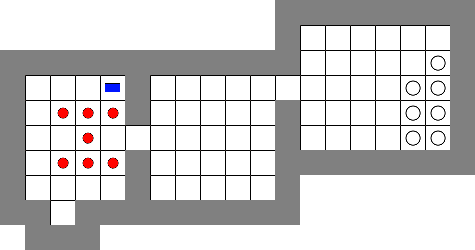
\includegraphics[scale=0.60]{./images/noDeadlocks.png}
\caption{A Sokoban map}
\end{figure}


From the computer science point of view, the game can be seen as a tree structure, the map configurations being the nodes and the original map acting as the root node. Thus, a solution state is the map where every goal square is covered by a box. The game's complexity derives from the high branching factor (the number of possible moves the player can make) and the enormous depth (some maps need more than 200 moves in order to be solved). Assuming an average branching factor of 2.5 (we rarely want to make a step back and a direction may be blocked), and a requirement of 100 moves to find the solution, we reach a complexity of $ 2.5^{100} $, well beyond today's computational capabilities. 

Our project focused mainly on implementing the informed best-first search algorithm and optimizing it as much as possible. Also, we have implemented a number of interesting methods like the push solver, or genetic algorithms.


  